\documentclass[a4paper,11pt]{article}
%\usepackage[T1]{fontenc}

%\setlength{\textwidth}{20cm}
%\setlength{\marginparwidth}{0cm}
%\setlength{\voffset}{0cm}
\usepackage[utf8]{inputenc}
\usepackage[francais]{babel}
\usepackage{amsmath}
\usepackage{graphicx}
\usepackage{listings}
\usepackage{color}
%==== to fix locations of figures and tables
\usepackage{float}
\usepackage{placeins}

\lstset{
language=VHDL,
basicstyle=\small\sffamily,
numbers=left,
numberstyle=\tiny,
frame=tb,
columns=fullflexible,
showstringspaces=false
}
%\special{papersize=210mm,297mm}

\title{{\Huge Electronique numérique}\\Initiation à VHDL (2/3)\\Circuits séquentiels. Automates.}
%\title{TD1}
\date{}

\begin{document}
\maketitle
Le TD précédent nous a permis de prendre en main VHDL, à travers des descriptions structurelles (instanciation de composants), ainsi que des équations logiques (assignations concurrentes).
 Nous poursuivons ici cette découverte du langage : nous allons notamment décrire des bascule D à l'aide du langage, et ainsi construire notre premier circuit séquentiel (un datapath simple).
Nous allons également découvrir deux manières de décrire des automates en VHDL :
\begin{itemize}
  \item En transposant directement les équations logiques des automates.
  \item Puis en reposant sur les capacités de synthèse du langage à un niveau plus élevé : le niveau RTL.
\end{itemize}

\section{Décrire des bascules D}
Nous avons vu précédemment que VHDL nous offre le moyen direct de décrire des équations logiques à l'aide d'assignations concurrentes. La partie droite d'une assignation concurrente peut
faire appel à des expressions à deux opérandes (expressions dites "binaires"...) comme le \textbf{and},\textbf{or},\textbf{not},\textbf{nor} etc...Ces opérations font partie intégrante
du langage : ce sont des mots clés de VHDL. La correspondance avec nos portes logiques
est donc immédiate. Malheureusement, ce n'est pas le cas pour la bascule D : il n'existe pas de mot clé pour décrire une telle bascule, de manière directe. Pour décrire les bascules D, il
est obligatoire de recourir à des \textbf{process}, au sein d'une \textbf{architecture}.

\begin{lstlisting}
entity a_circuit is
 port(
   reset_n : in std_logic;
   clk     : in std_logic;
   din     : in std_logic;
   qout    : out std_logic
 );
end entity;

architecture example of a_circuit is
begin

  -- ...

  bascule_d: process(reset_n,clk)
  begin
    if reset_n='0' then
      qout <= '0';
    elsif rising_edge(clk) then
      qout <= din;
    end if;
  end process;

  -- etc
  -- autres codes...

end example;

\end{lstlisting}

L'exemple précédent décrit une (seule) bascule D. On retiendra le gabarit de code qui conduit à créer (inférer est le terme exact) la bascule D. Quelques remarques s'imposent :
\begin{itemize}
  \item \textbf{Toute assignation concurrente sous le contrôle d'un front d'horloge génère une (ou plusieurs) bascule(s) D.}
  \item Le nommage de l'entrée D et de la sortie Q n'est pas obligatoire : on peut utiliser n'importe quels noms de signaux (pourvu qu'ils soient déclarés).
  Dans le jargon, on parlera alors de signaux "clockés".
  \item on peut utiliser n'importe quel {\it type} de signaux : \textbf{std\_logic}, \textbf{std\_logic\_vector(63 downto 0)}, \textbf{signed(31 downto 0)}, \textbf{unsigned(7 downto 0)}, mais également des types créés par l'utilisateur.
  \item Le caractère prioritaire du reset asynchrone (prioritaire par rapport à l'horloge) est ici manifeste dans le code (if ... elsif...).
  \item Le front montant se nomme ... \textbf{rising\_edge}.
  \item On peut coder plusieurs bascules D, à l'aide d'un seul processus, ou alors créer plusieurs processus. C'est au choix.
\end{itemize}

\section{Descriptions de chemin de données séquentiel}

Une relecture de l'énoncé du TD précédent rappelle que les opérateurs arithmétiques traditionnels sont crées automatiquement grâce aux symboles "+","-" etc,
dès lors que les données manipulées sont typées en \textbf{signed}
(par exemple \textbf{signed(7 downto 0)}) ou \textbf{unsigned(7 downto 0)}.

\boxed{Questions}
\begin{enumerate}
  \item Coder en VHDL au moins deux architectures numériques qui
  réalisent un compteur, qui compte de 0 à 255, en respectant l'entité donnée ci-dessous.
  On note que les opérandes sont codés en \textbf{unsigned(7 downto 0)} (octets non-signés);
  On prendra soin de \underline{dessiner} le circuit \underline{avant} de coder l'architecture.
  \item Tester le circuit à l'aide du testbench fourni.
\end{enumerate}

\begin{lstlisting}
library ieee;
use ieee.std_logic_1164.all;
use ieee.numeric_std.all;

entity compteur is
  port(
    reset_n : in  std_logic;
    clk     : in  std_logic;
    value   : out unsigned(7 downto 0)
  );
end compteur;
\end{lstlisting}


\section{Descriptions d'automates au niveau logique}
Soit un automate bien connu des informaticiens parisiens, sur la figure \ref{iloveparis}.

\begin{figure}
  \centering
  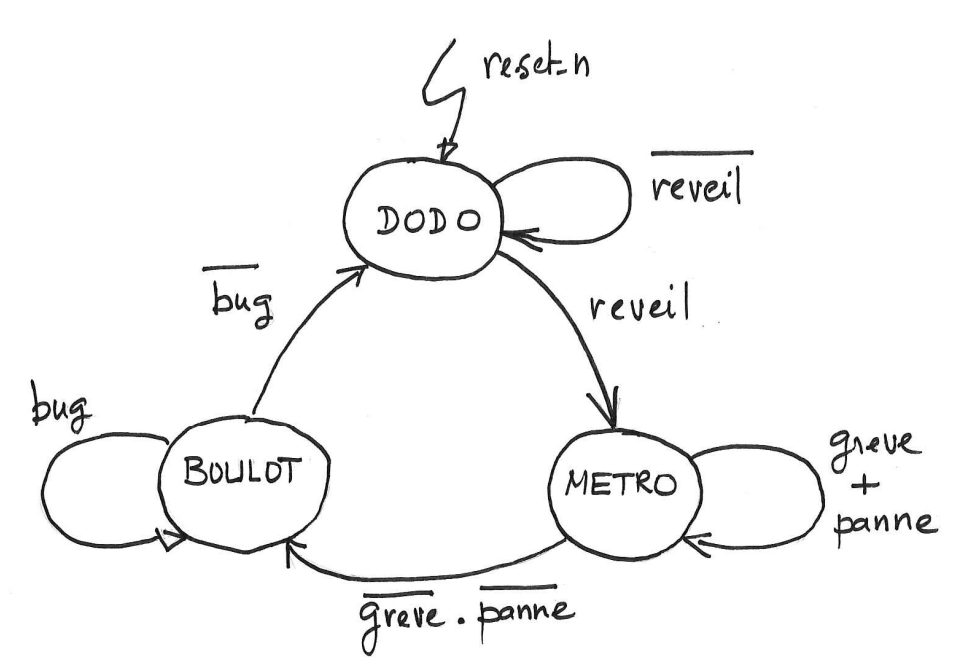
\includegraphics[width=8cm]{./iloveparis.png}
  \caption{Diagramme états-transitions de l'automate "I love Paris"}
  \label{iloveparis}
\end{figure}


\boxed{Questions}
\begin{enumerate}
  \item Vérifier que, dans le cas d'un encodage one-hot, les équations d'état suivant sont bien données par :

  $\left\{
  \begin{array}{rl}
    D_0 &= Q_0.\overline{reveil}+Q_2.\overline{bug} \\
    D_1 &= Q_0.reveil+Q_1.(greve+panne)\\
    D_2 &= Q_1.\overline{greve}.\overline{panne}+Q_2.bug\\
  \end{array}
  \right.$

  \item Coder l'automate "I\_love\_Paris" en VHDL, au niveau logique, en prenant soin de bien coder les bascules D à l'aide de processus.
  Respectez l'entité fournie ici. On utilisera une assignation conditionnelle (when) pour coder le signal de sortie "up\_and\_running".
  \lstset{inputencoding=utf8}
  \lstinputlisting[language=VHDL]{./code/i_love_paris_entity.vhd}
  %\item Ajouter un signal de sortie à votre convenance.\footnote{Sans signal de sortie, les synthétiseurs considèrent que la meilleure optimisation
  %consiste --à raison-- à générer un circuit absolument vide !}
  \item Utilisez le testbench donné sous Moodle pour tester votre automate. Observez le résultat.
\end{enumerate}

\section{Descriptions d'automates au niveau RTL}

Ce niveau d'abstraction RTL est le plus couramment utilisé, car il permet de
s'affranchir des détails des équations logiques, et décrire des automates (et {\it micro-architectures}) de manière plus naturelle.
Le niveau RTL repose sur la notion d'{\it inférence matérielle} : l'Electronicien doit connaître certains {\it motifs de conception}\footnote{"Design patterns", en anglais.}, afin
de permettre à l'outil de synthèse d'établir automatiquement les équations logiques sous-jacentes.
Le cas des automates d'états finis est instructif en ce sens. Voici un exemple
de codage VHDL, qui décrit un automate, sans expliciter les équations logiques sous-jacentes, ni l'encodage des états.
Pour information, le synthétiseur peut choisir de lui-même un encodage qui
maximise la fréquence de fonctionnement du circuit (encodage one-hot généralement),
ou tout autre type de contraintes imposées par le concepteur.

\paragraph{Exemple d'automate de niveau RTL}

Nous donnons ici à titre d'exemple un diagramme états-transitions, ainsi que son code VHDL de niveau RTL.
Notez que nous avons séparé le processus ici appelé "next\_state\_p", qui code
la fonction de transition (calcul de l'état suivant), et la sortie de l'automate.
\begin{center}
   \begin{minipage}[t]{8cm}
     \vspace{0pt}
     \lstset{inputencoding=utf8}
     \lstinputlisting[language=VHDL]{./code/automate.vhd}
   \end{minipage}%
   \begin{minipage}[t]{7cm}
     \vspace{40pt}
     \centering
     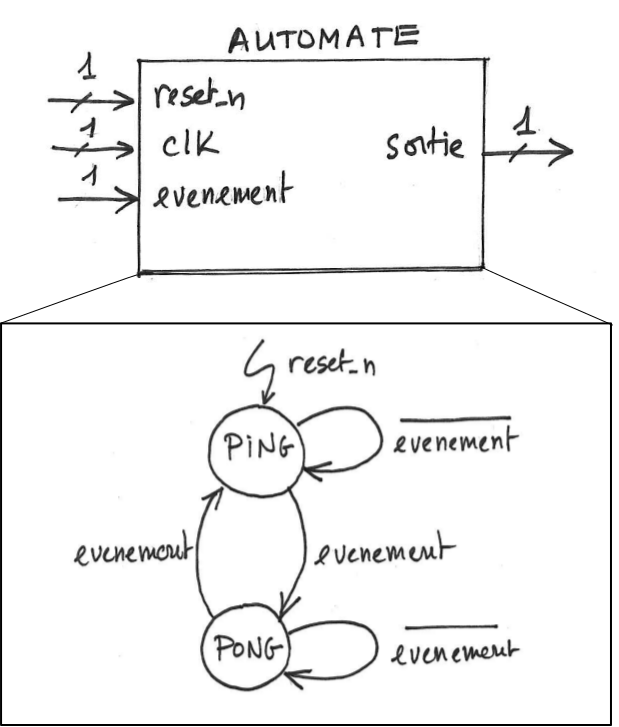
\includegraphics[width=6cm]{./ent_arch_ping_pong.png}
   \end{minipage}
\end{center} % added ending }

% \begin{minipage}[b]{15cm}
%   \lstset{inputencoding=utf8}
%   \lstinputlisting[language=VHDL]{./code/automate.vhd}
%   \begin{figure}
%     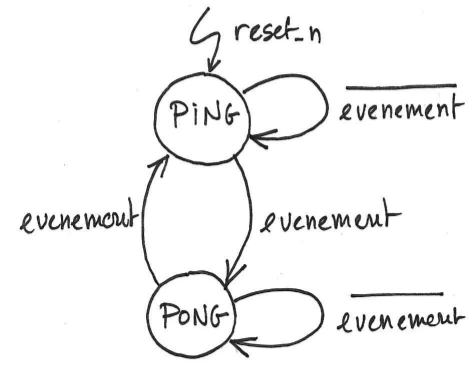
\includegraphics[width=8cm]{./ping_pong.png}
%     \caption{Diagramme états-transitions de l'automate "Ping-pong"}
%     \label{iloveparis}
%   \end{figure}
% \end{minipage}

\boxed{Questions}
\begin{enumerate}
  \item Prenez le temps de comprendre le codage utilisé ici.
  \item Coder l'automate "I\_love\_Paris" en VHDL, au niveau RTL, en vous inspirant de l'exemple donné.
  \item Utilisez le même testbench que précédemment pour tester votre automate. Modifier uniquement le nom de l'architecture associée à l'entité instanciée.
\end{enumerate}

\end{document}
